\section{Introduction}
For the group project we participated in the Right Whale Kaggle challenge where the aim is to create a face detector for the Right Whales \cite{kaggle2015}. This report details our attempt on building a classifier capable of indentifying 447 different Right whale individuals using deep learning techniques. 

\begin{wrapfigure}{l}[0pt]{0.4\textwidth}
	\vspace{-0.5cm}
	\centering
	
	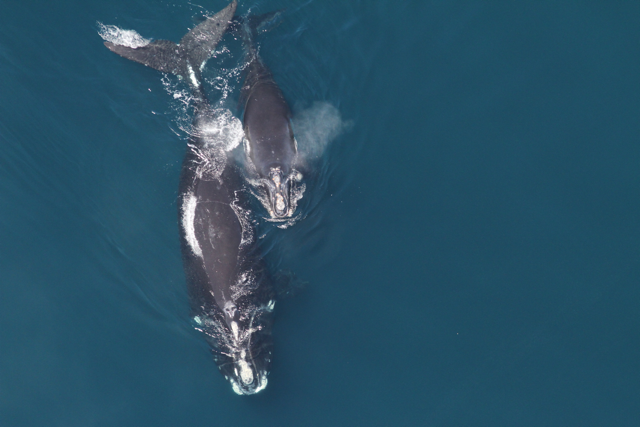
\includegraphics[width=0.4\textwidth]{sections/imgs/dataset/right_whale_example.png}
	\caption{Sample of a Right Whale}
	\label{fig:right_whale_sample}
	
	\vspace{-0cm}
\end{wrapfigure}

Overall we found the task challenging, mainly because the dataset was very sparse and the images given was noisy. Undesirable image properties includes variations in whale angles and sizes as well as large amount of water and waves hiding or covering the head of the whale, essential to identifying Right whales since the callosity pattern on top of a whale's head is unique for each whale (see Section \ref{sec:image_processing}).

As for the implementation we have chosen to use a library called Keras~\cite{keras2015}, a highly modular neural network library written in Python that uses Theano in the backend. In the following sections we detail how we prepared the dataset, the different techniques used to try and build a face detector for right whales, and experimental results from our attempts.